\begin{figure}[p]
\centering
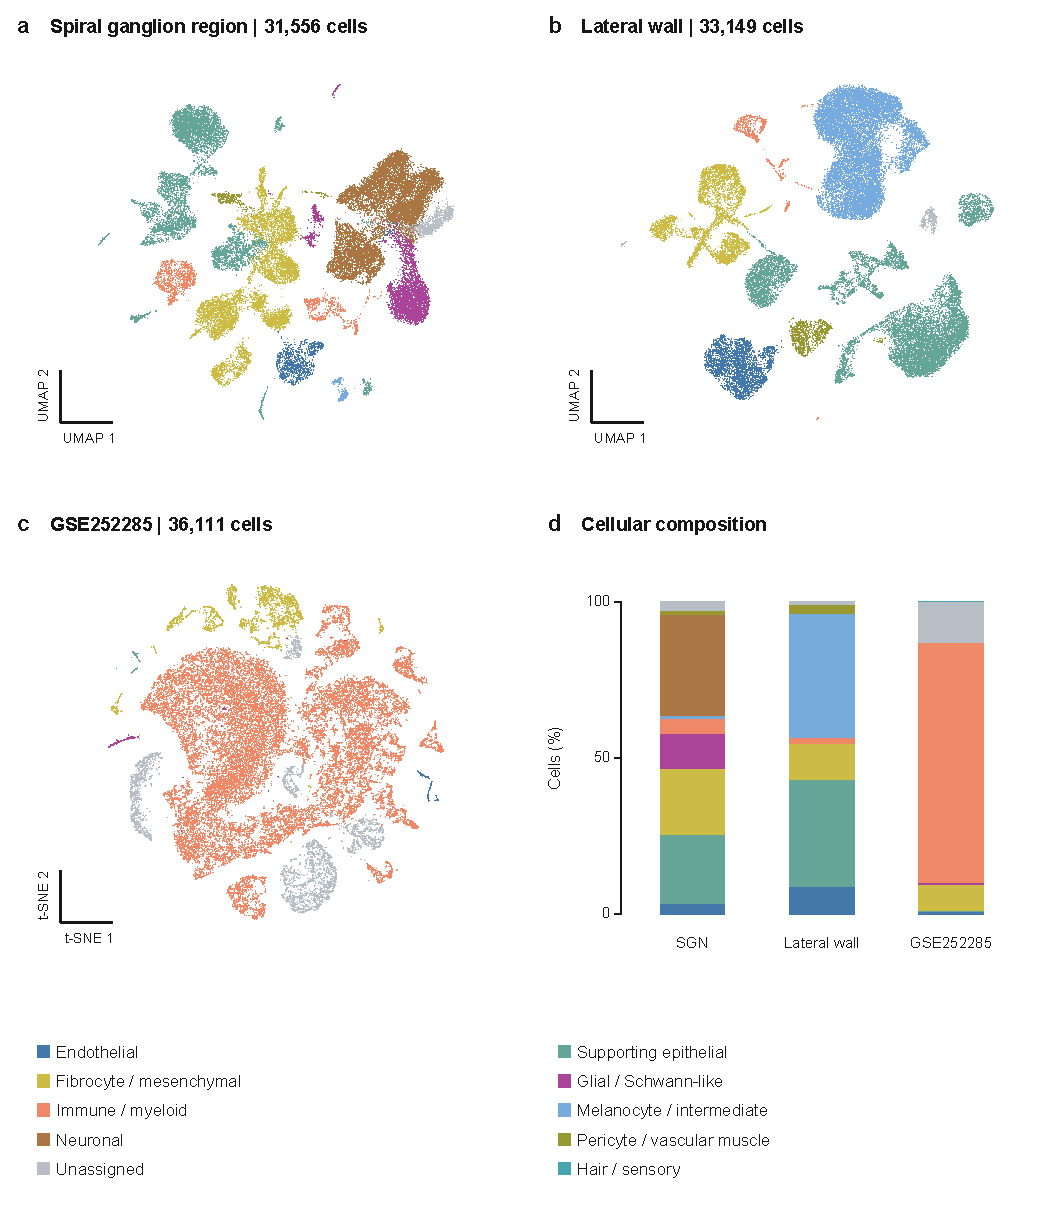
\includegraphics[width=\linewidth,height=0.74\textheight,keepaspectratio]{figures/Figure1_cell_atlases.pdf}
\caption{\textbf{Cochlear cell populations in the two single-cell datasets.} (a,b) UMAP projections of 31,556 spiral-ganglion-region cells and 33,149 lateral-wall cells from GSE168041, coloured by broad cell annotation. (c) The t-SNE projection of 36,111 GSE252285 cells using the selected resolution-0.6 clustering and primary broad annotations. Each point represents one cell. (d) Cell-type composition within the two GSE168041 compartments and GSE252285. Colours identify the same broad categories across panels; fractions use all retained cells as denominators. GSE168041 includes four naive and four noise-exposed samples per compartment. GSE252285 includes Control, HHL and NIHL libraries. SGN, spiral ganglion region; HHL, hidden hearing loss; NIHL, noise-induced hearing loss.}
\label{fig:1}
\end{figure}
\clearpage
\begin{figure}[p]
\centering
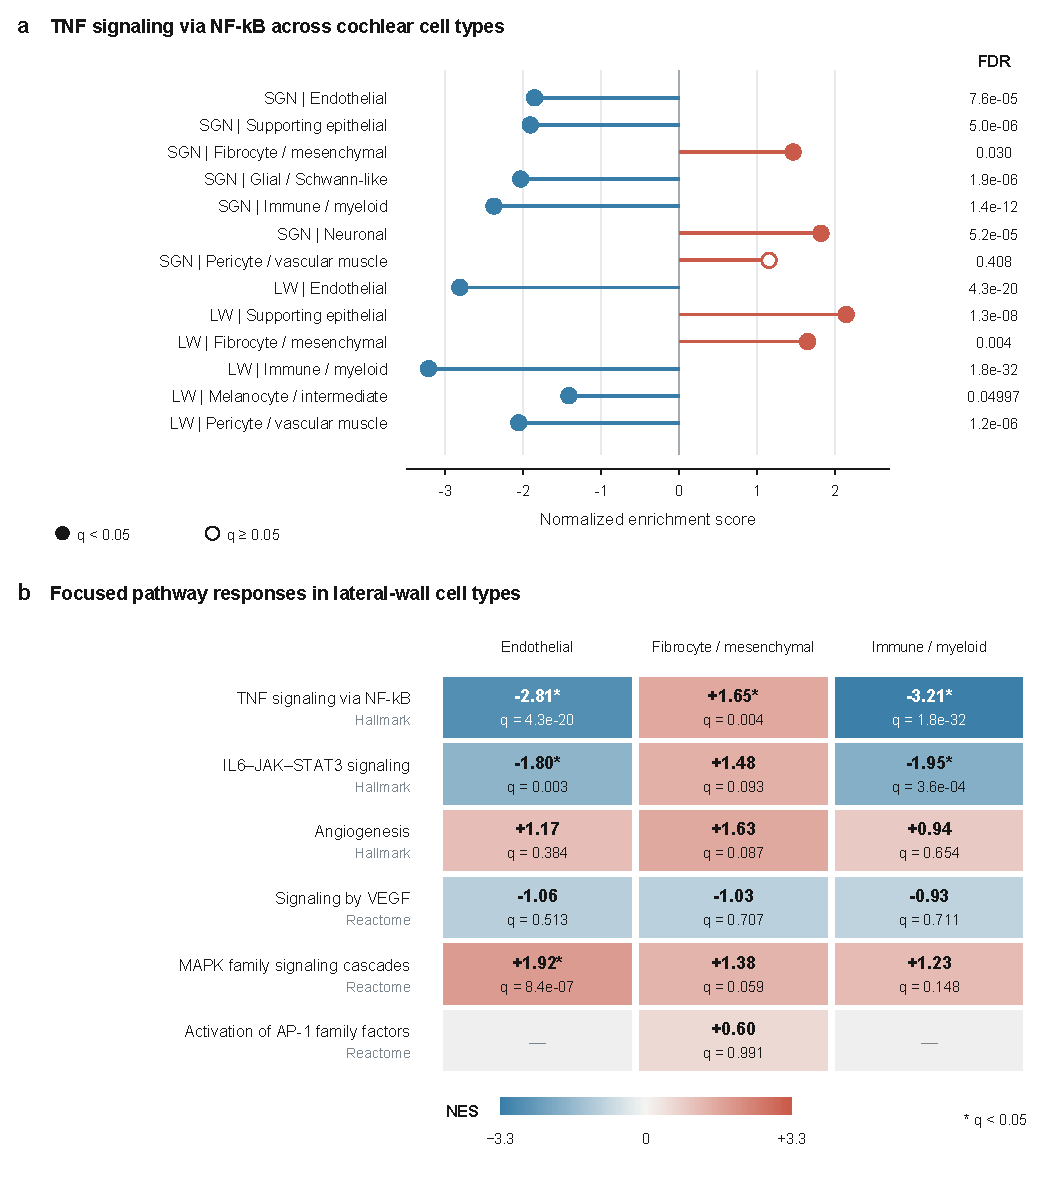
\includegraphics[width=\linewidth,height=0.72\textheight,keepaspectratio]{figures/Figure2_cell_type_pathway_responses.pdf}
\caption{\textbf{Cell-type-specific pathway responses to noise exposure.} (a) Normalized enrichment scores (NES) for the Hallmark TNF signaling via NF-\(\kappa\)B gene set across all thirteen eligible tissue--cell-type combinations in GSE168041. Filled points denote FDR \(<\) 0.05. Blue and red indicate enrichment toward naive and noise-exposed samples, respectively. The right-hand column gives FDR values. (b) NES and FDR values for six focused Hallmark and Reactome sets in lateral-wall endothelial, fibrocyte/\allowbreak{}mesenchymal and immune/\allowbreak{}myeloid cells. Asterisks identify FDR \(<\) 0.05; grey cells with a dash mark gene sets outside the eligible size range. Hallmark angiogenesis, Reactome VEGF signaling, Reactome MAPK family signaling cascades and Reactome AP-1 activation are reported separately. Each sample-level pseudobulk contrast used four naive and four noise-exposed samples. LW, lateral wall; SGN, spiral ganglion region.}
\label{fig:2}
\end{figure}
\clearpage
\begin{figure}[p]
\centering
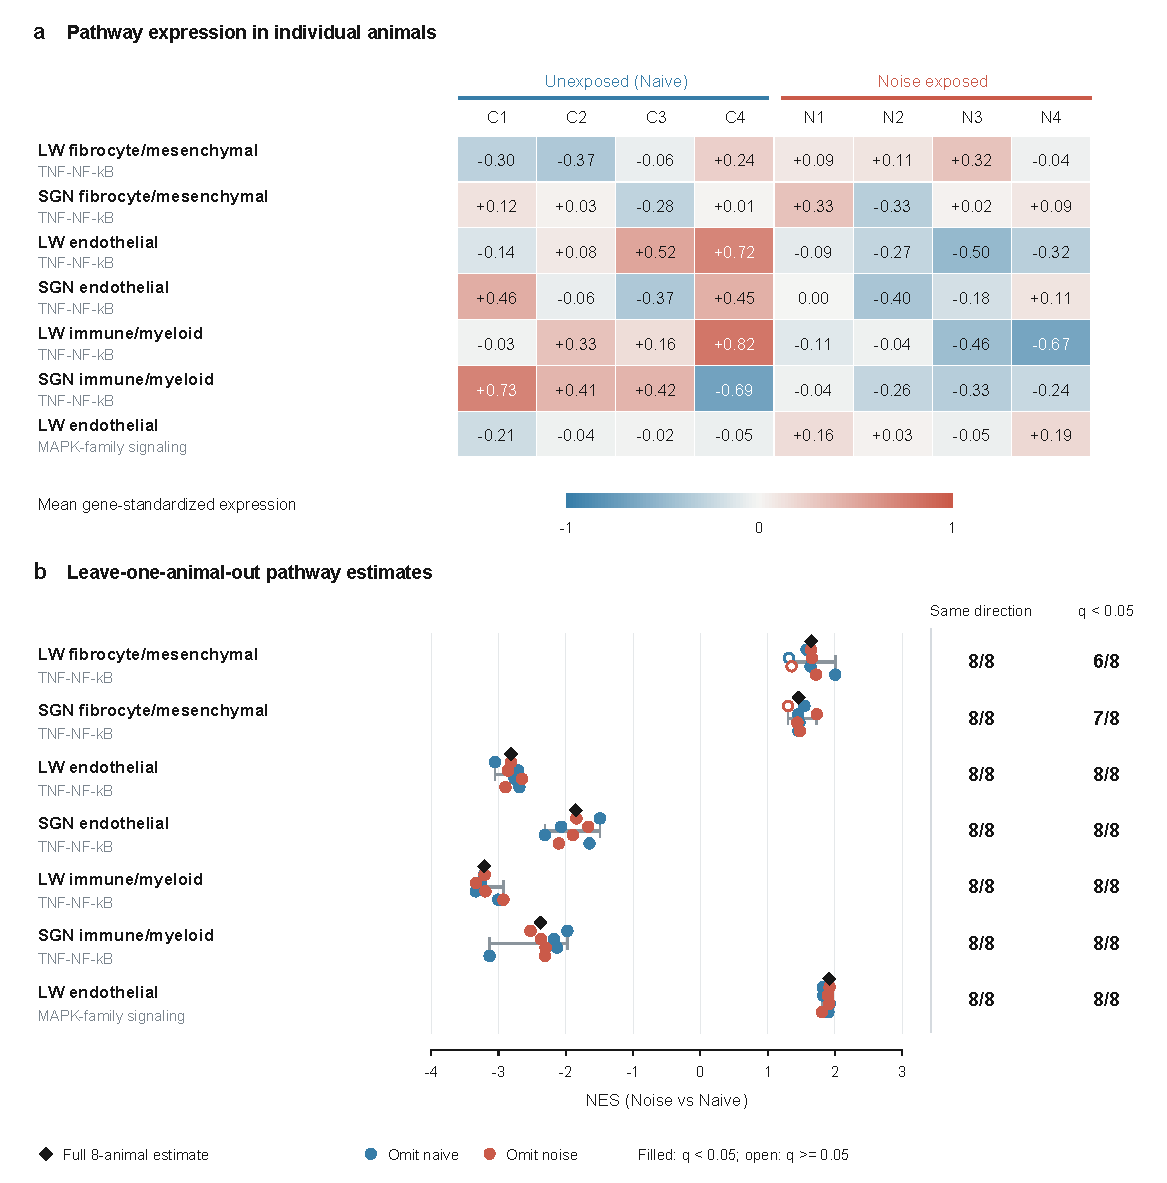
\includegraphics[width=\linewidth,height=0.74\textheight,keepaspectratio]{figures/Figure3_sample_robustness.pdf}
\caption{\textbf{Individual-sample profiles and sensitivity of the core pathway responses.} (a) Standardized pathway-expression profiles for the six TNF--NF-\(\kappa\)B tissue--cell-type combinations and lateral-wall endothelial MAPK signaling. Normalized pseudobulk counts were log1p-transformed, standardized within each gene across the eight samples, and averaged over the fixed mapped pathway members. C1--C4 and N1--N4 denote naive and noise-exposed samples, respectively; codes are indexed separately within each tissue. (b) Full-sample and leave-one-sample-out NES estimates for the same seven pathway--model combinations. Each model used all eight samples for its main estimate and seven samples for each of eight omissions. Black diamonds show the full-sample estimates. Blue and red circles denote omission of a naive or noise-exposed sample, respectively; filled circles mark FDR \(<\) 0.05. Horizontal lines show the minimum-to-maximum range of the eight omission estimates. The columns report direction agreement with the full model and the number of omission fits with FDR \(<\) 0.05. All originally eligible Hallmark and Reactome sets were included in each model's multiple-testing family. LW, lateral wall; SGN, spiral ganglion region; NES, normalized enrichment score; FDR, false discovery rate.}
\label{fig:3}
\end{figure}
\clearpage
\begin{figure}[p]
\centering
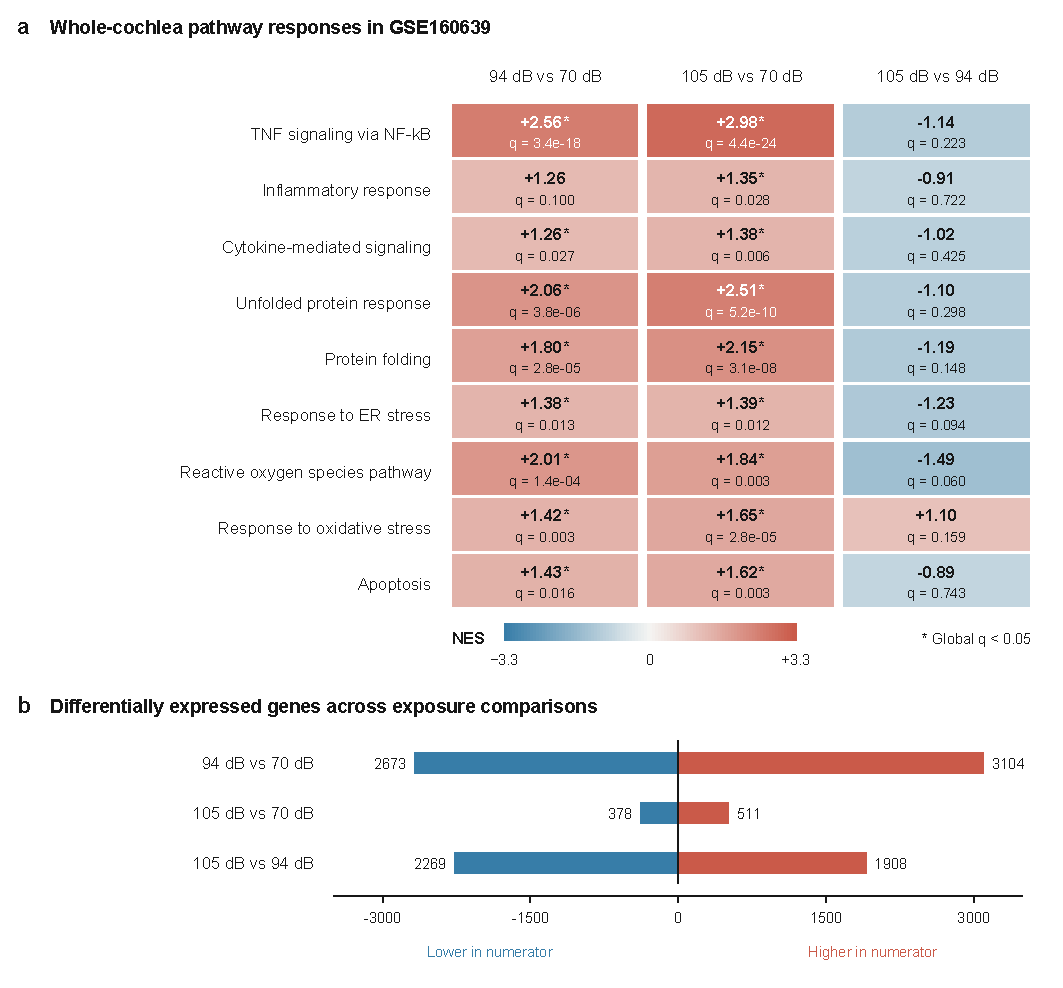
\includegraphics[width=\linewidth,height=0.72\textheight,keepaspectratio]{figures/Figure4_noise_exposure_comparisons.pdf}
\caption{\textbf{Whole-cochlea transcriptional responses across noise exposures.} (a) All nine targeted gene sets across the three GSE160639 exposure comparisons, estimated from raw-count DESeq2 contrasts. Each tile reports the normalized enrichment score (NES) and the Benjamini--Hochberg FDR adjusted jointly across all 27 tests. Positive NES indicates enrichment toward the first exposure in the stated comparison. Asterisks identify global FDR \(<\) 0.05. Hallmark sets comprise TNF signaling via NF-\(\kappa\)B, inflammatory response, unfolded protein response, reactive oxygen species pathway and apoptosis; the remaining sets are Gene Ontology Biological Process terms. (b) Gene counts at FDR \(<\) 0.05 from DESeq2 Wald tests, with blue and red bars denoting lower and higher expression in the numerator exposure. No additional fold-change threshold was applied. Gene-level and pathway-level FDR values refer to their respective multiple-testing families.}
\label{fig:4}
\end{figure}
\clearpage
\begin{figure}[p]
\centering
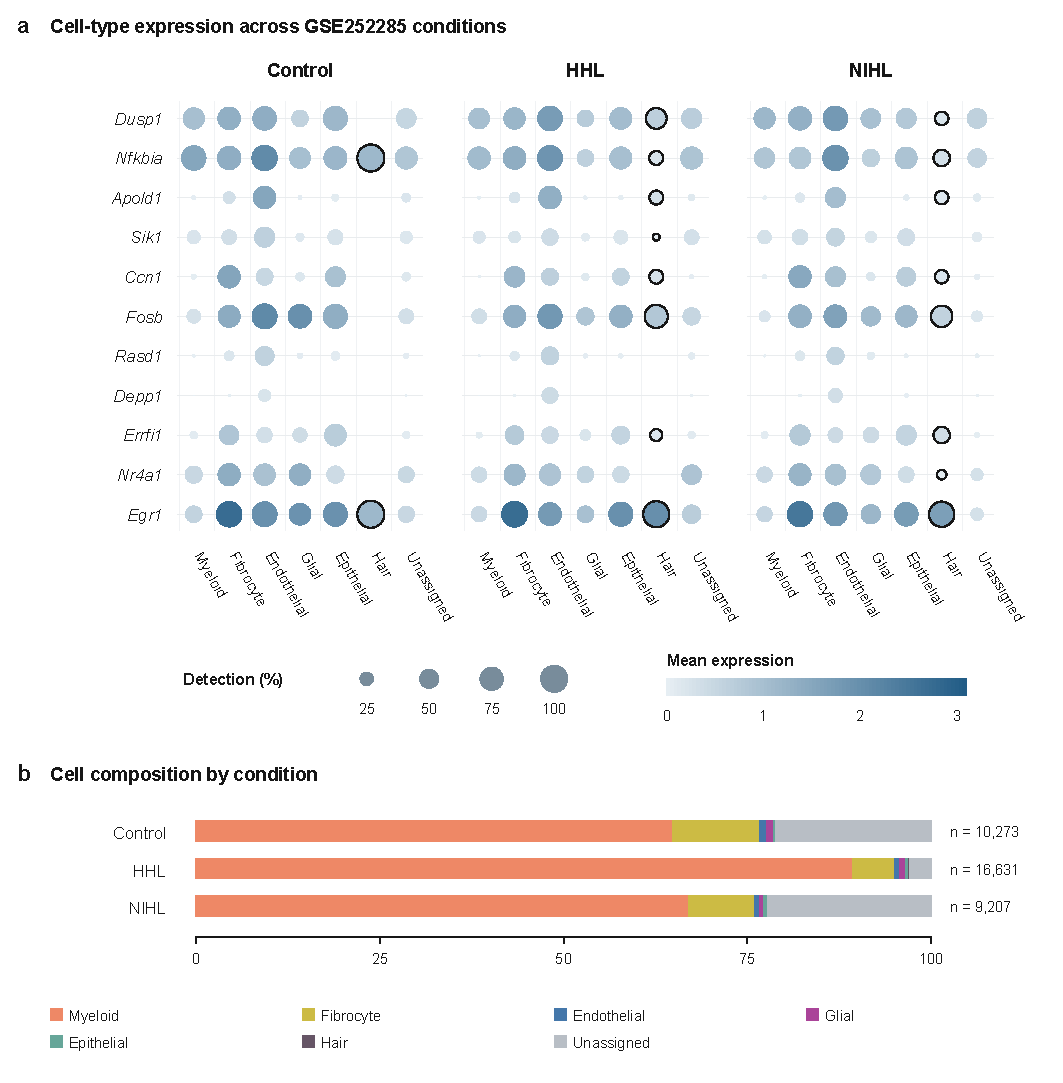
\includegraphics[width=\linewidth,height=0.72\textheight,keepaspectratio]{figures/Figure5_condition_expression.pdf}
\caption{\textbf{Condition-resolved expression of genes with stable cell-type localization.} (a) Eleven genes whose highest-ranked broad cell type by mean normalized expression (with detection fraction used to break ties) was retained across Control, HHL and NIHL conditions in GSE252285, with at least 20 cells in each top-ranked group. Dot area represents the percentage of cells with RNA counts greater than zero. Colour represents mean normalized expression across all cells in each group, including zeros, on a shared scale. Outlined dots identify groups containing fewer than 20 cells. (b) Broad cell-type composition and cell counts in the three condition libraries. The three libraries contain 36,111 cells, summarized using their existing clusters and annotations. Fibrocyte, epithelial and hair labels denote fibrocyte/mesenchymal, supporting/epithelial and hair/sensory populations, respectively. HHL, hidden hearing loss; NIHL, noise-induced hearing loss.}
\label{fig:5}
\end{figure}
\clearpage
\begin{figure}[p]
\centering
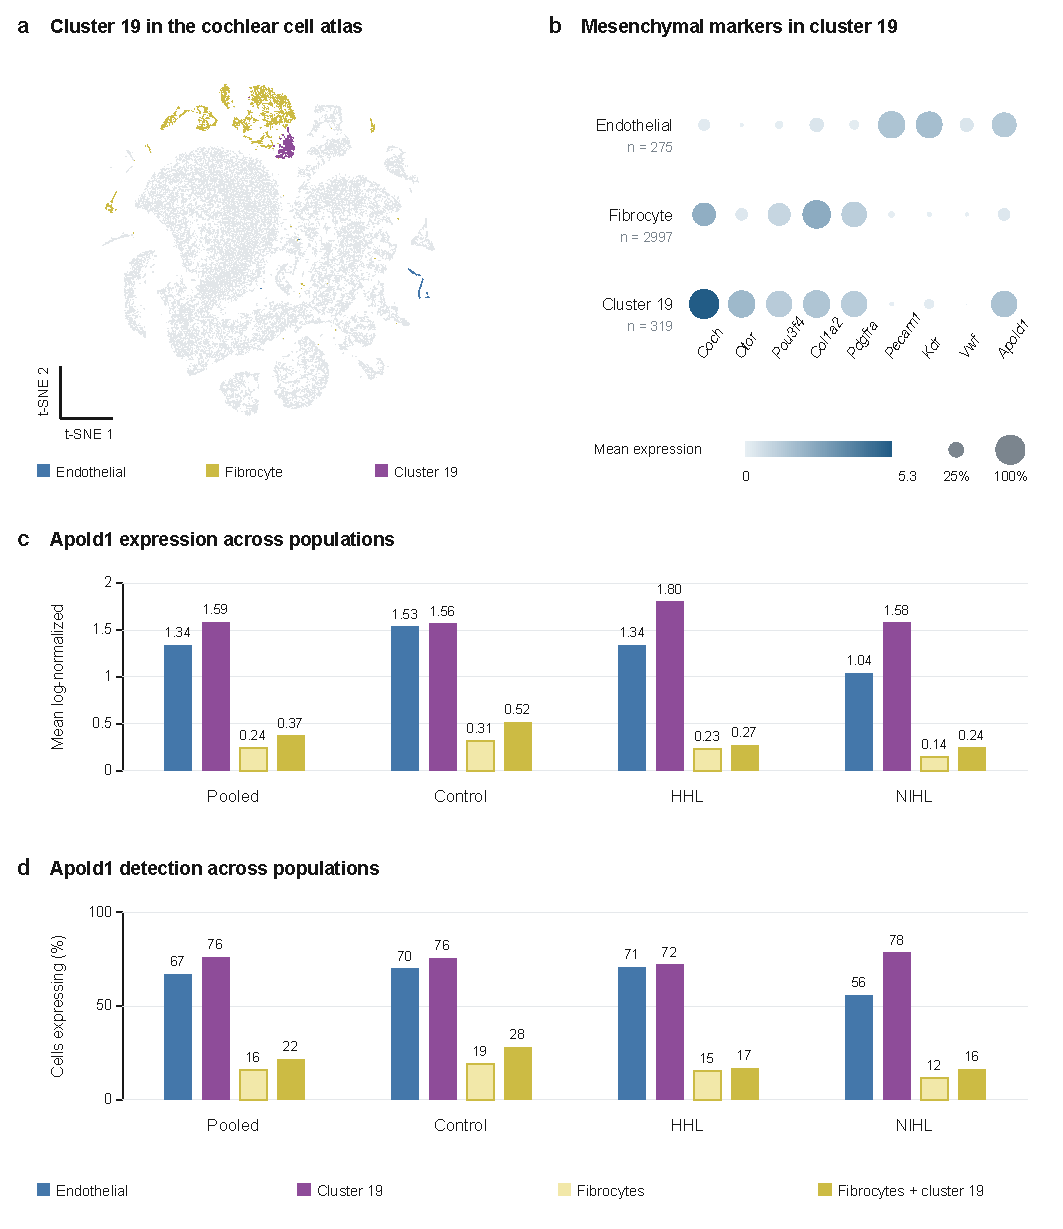
\includegraphics[width=\linewidth,height=0.74\textheight,keepaspectratio]{figures/Figure6_cluster19_expression.pdf}
\caption{\textbf{Cluster 19 expresses mesenchymal markers and contributes to \textmd{\textit{Apold1}} expression.} (a) The fixed GSE252285 t-SNE projection highlights primary endothelial and fibrocyte/mesenchymal populations and the 319 cells in cluster 19. (b) Canonical-marker expression in endothelial cells, primary fibrocyte/mesenchymal cells and cluster 19. Dot area denotes the detection fraction, and colour denotes mean log-normalized expression on a shared scale. (c,d) Mean log-normalized \textit{Apold1} expression and detection fractions in pooled cells and each library. Primary fibrocyte/mesenchymal summaries exclude cluster 19; the reassigned summaries include its 319 cells. Cluster 19 is also shown separately to retain its distinct expression profile. Endothelial summaries use the same 275 cells under both annotation schemes. Each bar summarizes cells within its stated group. HHL, hidden hearing loss; NIHL, noise-induced hearing loss.}
\label{fig:6}
\end{figure}
\clearpage
